% !TEX ROOT = ../ersti.tex

\section{Wohnen in Heidelberg}

Wie in jeder Unistadt, so ist es auch in Heidelberg schwer, zu Anfang des Semesters ein Zimmer zu finden, das bezahlbar ist und möglichst zentral liegt. Im Durchschnitt muss man in Heidelberg mit Lebenshaltungskosten von ca. \lebenshaltungskosten (inklusive Miete) pro Monat rechnen.

\begin{figure*}[t]
    \centering
    \begin{subfigure}{.3\textwidth}
    
\includegraphics[height=4.5cm]{bilder/travelling_salesman_problem_1.png}
    \end{subfigure}
    \begin{subfigure}{.3\textwidth}
    
\includegraphics[height=4.5cm]{bilder/travelling_salesman_problem_2.png}
    \end{subfigure}
    \begin{subfigure}{.3\textwidth}
    
\includegraphics[height=4.5cm]{bilder/travelling_salesman_problem_3.png}
    \end{subfigure}
\end{figure*}

Am günstigsten wohnt man immer noch im Studierendenwohnheim, dort muss man mit Mieten von ca.~\studentenwohnheim pro Monat rechnen. Eine frühzeitige Bewerbung ist hier dringend notwendig. Auch WG-Zimmer sind teilweise recht günstig zu bekommen, in der Regel jedoch teurer als ein Zimmer im Wohnheim und oft nicht lange im Voraus zu reservieren.

Die Idee, eine eigene WG zu gründen, liegt meist sehr nahe, jedoch wird man schnell merken, dass das gar nicht so einfach ist. Oft werden Ehepaare ohne Kinder bevorzugt oder ein Zimmer entpuppt sich als Durchgangszimmer. Egal für was ihr euch entscheidet: Plant viel Zeit ein und lasst nicht locker!

Nun aber zur konkreten Zimmersuche: Es gibt mehrere Möglichkeiten, ein Zimmer in Heidelberg zu finden. Das Studierendenwerk bietet mehrere Anlaufstellen: In der Altstadt das Info-Café International in der Triplex-Mensa direkt am Uniplatz, im Neuenheimer Feld im Infocenter der Zentralmensa. In den Mensen, aber auch in den einzelnen Instituten empfiehlt es sich, die schwarzen Bretter abzuklappern und nach privaten Aushängen Ausschau zu halten oder selbst Anfragen anzuhängen. Weitere gute Quellen für Zimmerangebote sind natürlich die regionalen Zeitungen. Das wären u.a. \emph{Sperrmüll}, erscheint immer dienstags und freitags und die Rhein-Neckar-Zeitung, mittwochs und samstags mit großem Immobilienteil. %Aufpassen müsst ihr bei Makler-Vermittlungen, hier müsst ihr zusätzlich zwischen %ein und zwei Monatsmieten Provision zahlen. Eine eigene Anzeige kann natürlich nie schaden. Zu guter Letzt gibt es noch das Internet, das eine Fülle an Portalen\footnote{z.B. \url{wg-gesucht.de}} zur Wohnungssuche bietet.


\subsubsection{Wohnheime}

%\begin{figure*}[t]
%    \centering
%    \begin{subfigure}{.2\textwidth}
%    
\includegraphics[height=4.5cm]{bilder/household_tips_1.png}
%    \end{subfigure}
%    \begin{subfigure}{.25\textwidth}
%    
\includegraphics[height=4.5cm]{bilder/household_tips_2.png}
%    \end{subfigure}
%    \begin{subfigure}{.2\textwidth}
%    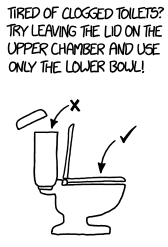
\includegraphics[height=4.5cm]{bilder/household_tips_3.png}
%    \end{subfigure}
%    \begin{subfigure}{.28\textwidth}
%    
\includegraphics[height=4.5cm]{bilder/household_tips_4.png}
%    \end{subfigure}
%\end{figure*}

In und um Heidelberg gibt es ca. 50 Wohnheime des Studierendenwerks, im Wintersemester werden ca. ein Fünftel aller dieser Zimmer neu vermietet. Die Auswahl erfolgt nach sozialen Kriterien wie zum Beispiel Heimatferne, Verdienst der Eltern, Wohnverhältnisse usw. Die Wohnzeit ist auf sechs Semester begrenzt, aber es gibt viele Möglichkeiten, diese zu verlängern, zum Beispiel durch Sonderaufgaben im Wohnheim, Härtefälle, Engagement in der Fachschaft, etc. Die maximale Wohnzeit kann auf insgesamt zehn Semester ansteigen, was durchaus vorkommt. Je nach Wohnheim gibt es Einzelzimmer mit Stockwerksküche und -bad, die ihr dann mit jeweils 15-20 Leuten teilt -- was mittlerweile aber eher selten ist -- Einzelzimmer in 2er, 3er oder 4er WGs oder sogar Einzelappartments. Die Zimmer sind in der Regel nicht sehr groß (11--16 \squaren\metre), aber ausreichend. Nachteile von Wohnheimen können die teilweise sehr unterschiedlichen Vorstellungen von Hygiene sein, ein hoher Lärmpegel und immer wieder neue Überraschungen. Allerdings bietet ein Wohnheim vor allem für Leute, die neu in der Stadt sind, den großen Vorteil, sehr schnell viele Leute kennen zu lernen, außerdem muss man sich um Reparaturen nicht selbst kümmern. Es gibt keine konkreten Bewerbungsfristen. Die Bewerbung sollte allerdings bis 1. Juli für das Wintersemester und bis 1. Januar für das Sommersemester eingegangen sein, weil dann mit der Zimmereinteilung und dem Versand der Mietverträge begonnen wird. Später eingehende Bewerbungen haben weitaus geringere Chancen und Auswahlmöglichkeiten. Antragsformulare gibt es in den Infocentern des Studierendenwerks oder im Internet\footnote{\url{http://www.studentenwerk.uni-heidelberg.de}}. Dort gibt es auch eine vollständige Liste aller Wohnheime des Studierendenwerks. Auch private, kirchliche oder sonstige Träger bieten Zimmer in Wohnheimen an, für diese müsst ihr euch direkt beim Wohnheim bewerben, nicht beim Studierendenwerk. Eine Liste findet ihr aber beim Studierendenwerk\footnote{\url{http://www.stw.uni-heidelberg.de/sites/default/files/download/pdf/wo-in-hd-andere-traeger-de.pdf}}.
